\documentclass[tikz]{standalone}

\ifdefined\STANDALONE  % Check if macro is defined.
\else
	\providecommand{\STANDALONE}{}
\fi

\begin{document}
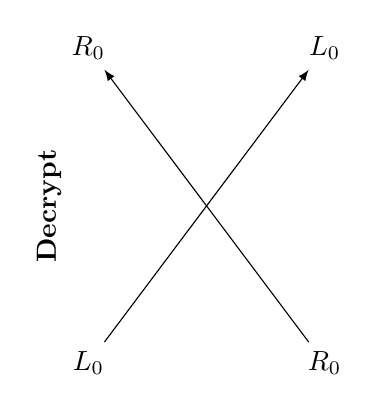
\begin{tikzpicture}

	% Node definitions.
	\node  (ip_left) at (0,0) {$L_0$};
	\node (ip_right) at (3,0) {$R_0$};
	\node  (r1_left) at (0,4) {$R_0$};
	\node (r1_right) at (3,4) {$L_0$};

	% Arrows.
    \draw[-latex] (ip_right) -- (r1_left);
	\draw[-latex]  (ip_left) -- (r1_right);

    % Title.
    \node[rotate=90] at (-0.5,2) {\textbf{Decrypt}};

\end{tikzpicture}
\end{document}